\subsection{Estación de alta densidad}

A medida que mas ramales ferroviarios coexisten en la misma línea se vuelve inevitable que varias líneas compartan la misma estación utilizando diferentes plataformas en paralelo. Con una logística mas flexible, las diferentes líneas incluso pueden utilizar de forma alternada las mismas plataformas y, por lo tanto, las mismas vías principales. Además, es necesario contar con mecanismos para retirar trenes de la red para su mantenimiento y volver a inyectarlos a la red cuando la demanda aumente. Esto se logra por medio de talleres ferroviarios en las inmediaciones de las estaciones que actúan como un hub ferroviario. La topología de estación de alta densidad se ilustra en la Figura \ref{fig:hub_1}.

    \begin{figure}[h]
        \centering
        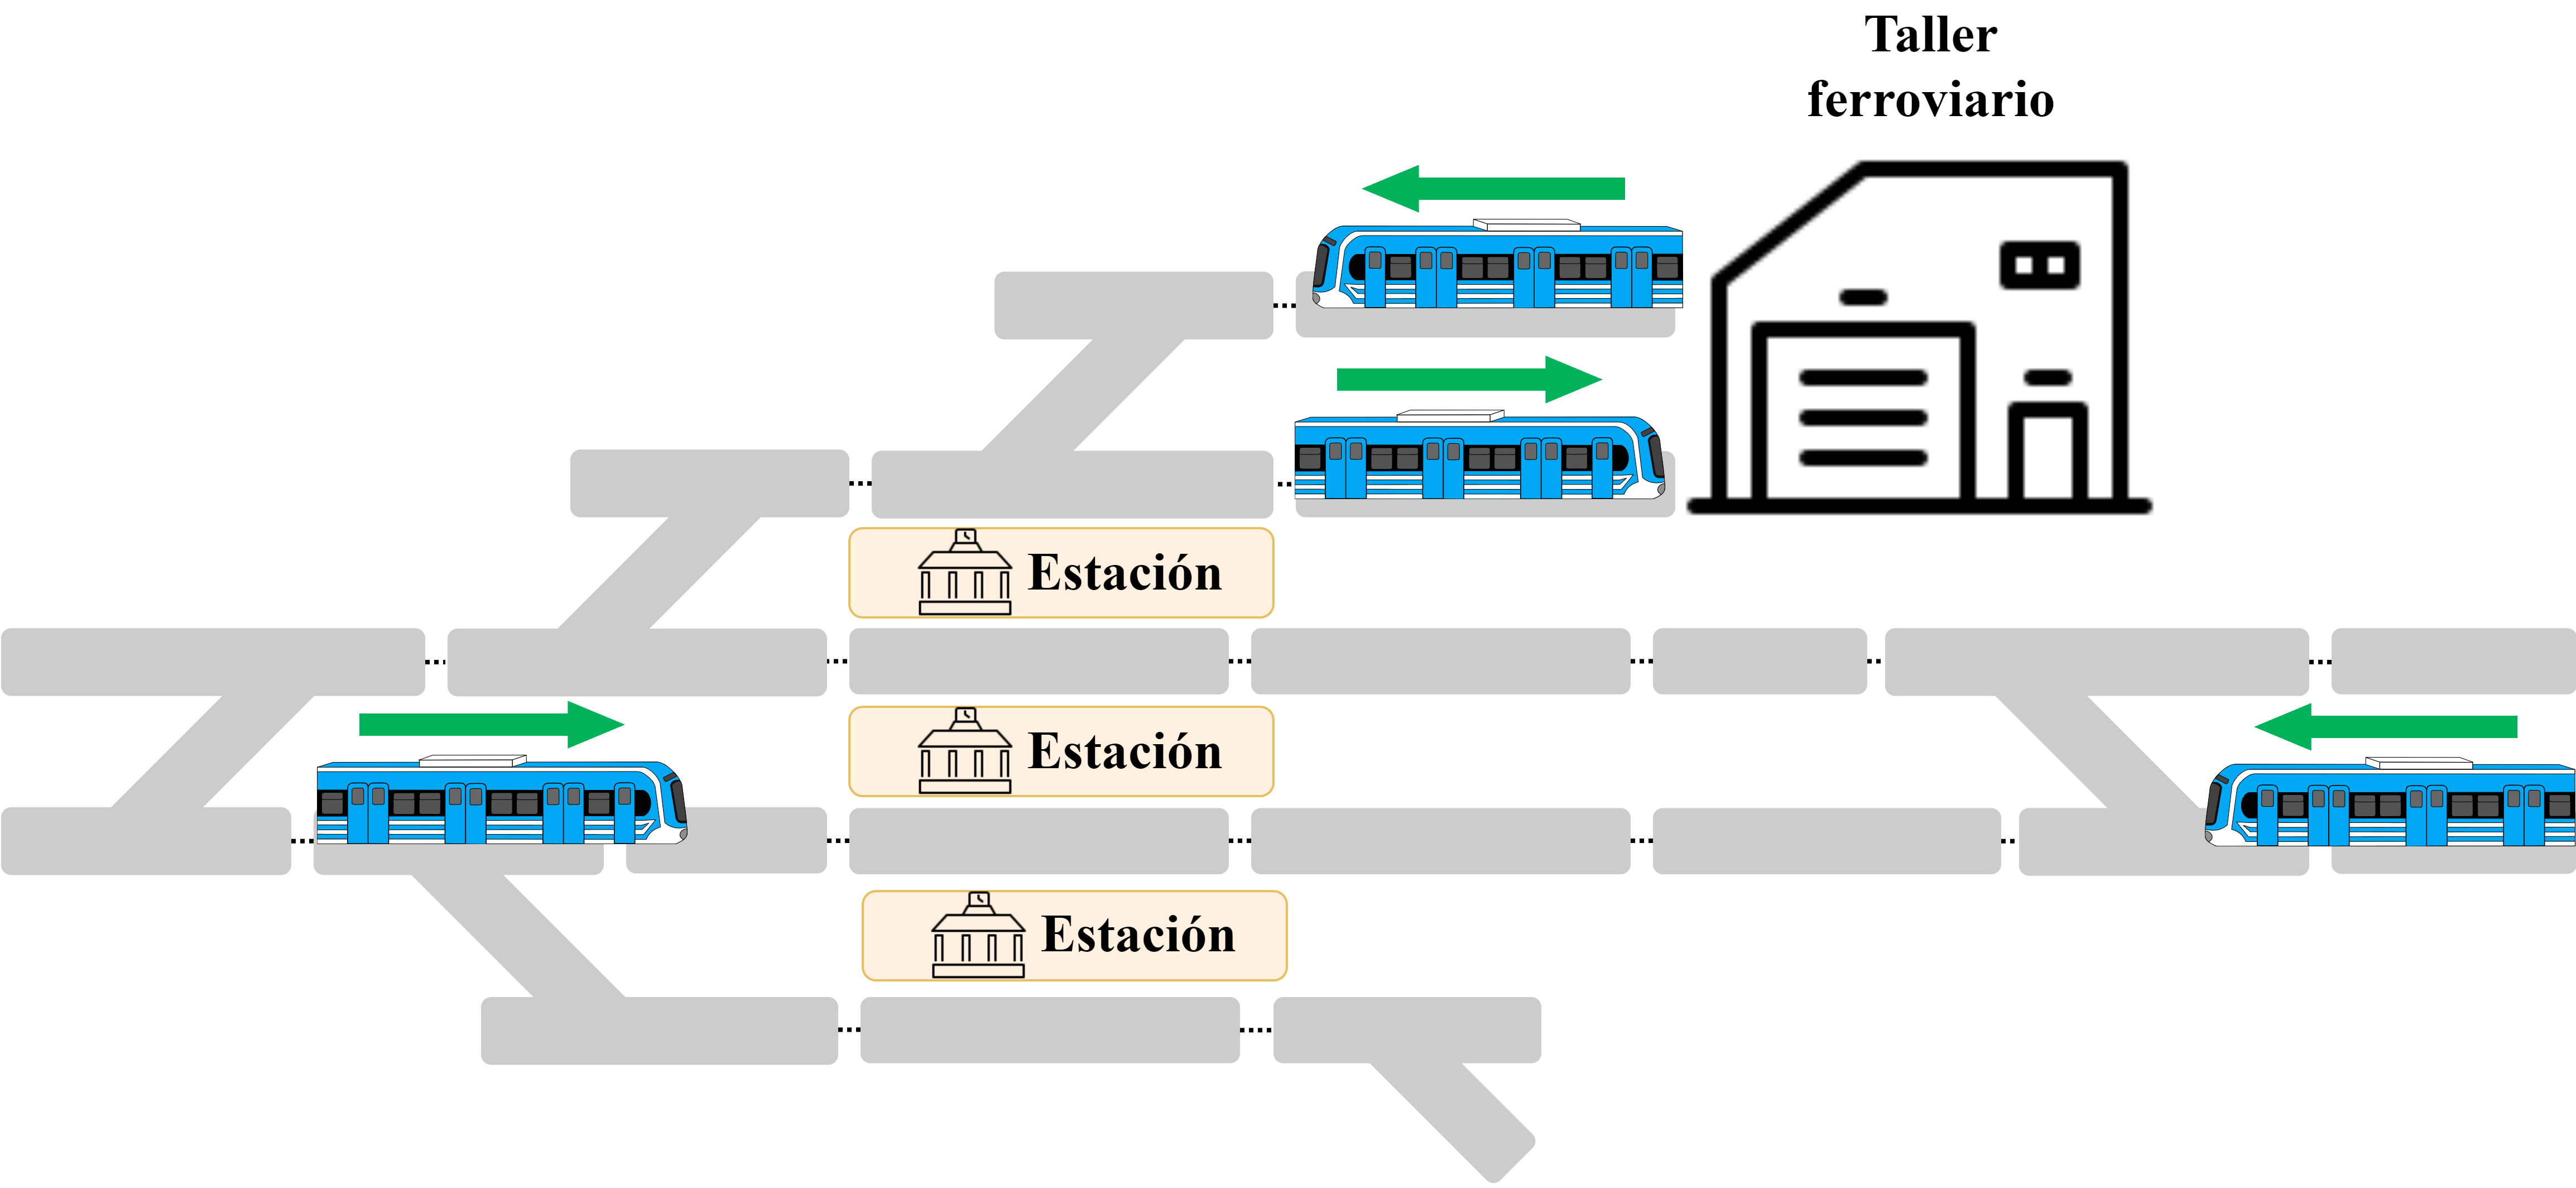
\includegraphics[width=1\textwidth]{Figuras/altaDensidad}
        \centering\caption{Topología de Estación de alta densidad.}
        \label{fig:hub_1}
    \end{figure}
    
%Las tareas del sistema de enclavamientos van aumentando en complejidad a medida que se suman nuevos elementos ferroviarios. Debe coordinar diversas formaciones de distintas líneas, accediendo a diferentes plataformas, cumpliendo diferentes horarios de arribo y partida. A su vez, debe asegurarse de que las formaciones circulen con seguridad pero sin descuidar la puntualidad. Adicionalmente, debido a que la demanda varía a lo largo del día, deberá tener flexibilidad para inyectar nuevas formaciones a la red o remover las que presenten desperfectos técnicos. Todas estas acciones deben realizarse en simultáneo y en un entorno de alto dinamismo.

Las tareas del sistema de enclavamientos van aumentando en complejidad a medida que se suman nuevos elementos ferroviarios. Por ejemplo, debe segurar que las formaciones circulen con seguridad pero sin afectar la disponibilidad del sistema. %Adicionalmente, debido a que la demanda varía a lo largo del día, deberá tener flexibilidad para inyectar nuevas formaciones a la red o remover las que presenten desperfectos técnicos. Todas estas acciones deben realizarse en simultáneo y en un entorno de alto dinamismo.